\documentclass[11pt]{article}

\usepackage[margin=1in]{geometry}
\usepackage{amsmath}
\usepackage{booktabs}
\usepackage{array}
\usepackage{siunitx}
\usepackage[T1]{fontenc}
\usepackage{tikz}
\usepackage{pgfplots}
\usepgfplotslibrary{groupplots}
\usepackage{pgfplotstable}
\usepackage{caption}
\captionsetup{font=small,width=0.92\textwidth}
\usepackage{hyperref}
\usepackage{float}
\usepackage{xcolor}
\usetikzlibrary{arrows.meta,positioning,calc,fit,matrix}
\pgfplotsset{compat=1.18}
\sisetup{detect-all}

\definecolor{adcblue}{RGB}{30,74,138}
\definecolor{adcred}{RGB}{158,40,47}
\definecolor{adcgreen}{RGB}{31,119,86}
\definecolor{adcorange}{RGB}{217,119,6}
\definecolor{adcpurple}{RGB}{93,63,211}
\definecolor{adcgray}{RGB}{90,90,90}

\begin{document}
\begin{titlepage}
\centering
\vspace*{1.8cm}
{\Huge \bfseries Project Report\par}
\vspace{0.45cm}
{\Large ELEC 5705\par}
\vspace{0.7cm}
{\Large Behavioral Reimplementation of a\\Background-Calibrated 13-bit SAR ADC\par}
\vfill
{\Large Jesse Levine\par}
\vspace{0.3cm}
{\large 101185127\par}
\vspace{1.2cm}
{\large April 2026\par}
\end{titlepage}

\begin{abstract}
This project reimplements the background calibration architecture of the 46~\si{\micro\watt}, 13-bit, 6.4~MS/s SAR ADC reported by Ding \emph{et al.} using a hybrid methodology. The ADC core, DAC mismatch, comparator modes, and analog correction path are modeled behaviorally, while the sign extraction and immediate calibration-control path are implemented explicitly in RTL. The final model reproduces sparse background operation and converges in 384243 conversions with an active calibration rate of approximately 1.37\%, close to the paper's reported convergence scale of roughly 400k cycles.
\end{abstract}

\section{Objective}
The paper \cite{ding2017} uses redundancy and a sign-based background calibration loop to suppress DAC mismatch and comparator dynamic offset while keeping the ADC power very low. The project target was to reimplement that calibration architecture without going transistor-level. Following the project guidance, the implementation split used here is:
\begin{itemize}
    \item behavioral modeling for the ADC core and analog correction plant, and
    \item explicit RTL for the sign-extraction path and the immediate calibration-control logic.
\end{itemize}

This yields a model that still captures the paper's \cite{ding2017} central contribution: the calibration loop only needs the \emph{sign} of the error, not a full digital estimation engine.

In practical terms, the project focuses effort where the calibration architecture is most distinctive. The converter front end is kept at the behavioral level so that mismatch, redundancy, and comparator-mode effects can be exercised over long simulations, while the calibration decision path is forced to exist as real logic that captures trigger interpretation, sign extraction, filtering, and trim update.

\section{Architecture}
Figure~\ref{fig:top_arch} shows the overall project partition. The behavioral side produces the internal raw code and the modeled comparator/DAC behavior. The explicit RTL side interprets calibration triggers, extracts the sign from $D_{15}$ and $D_{16}$, filters the sign decisions through a 6-bit bidirectional counter, and updates the trim registers.

\begin{figure}[H]
\centering
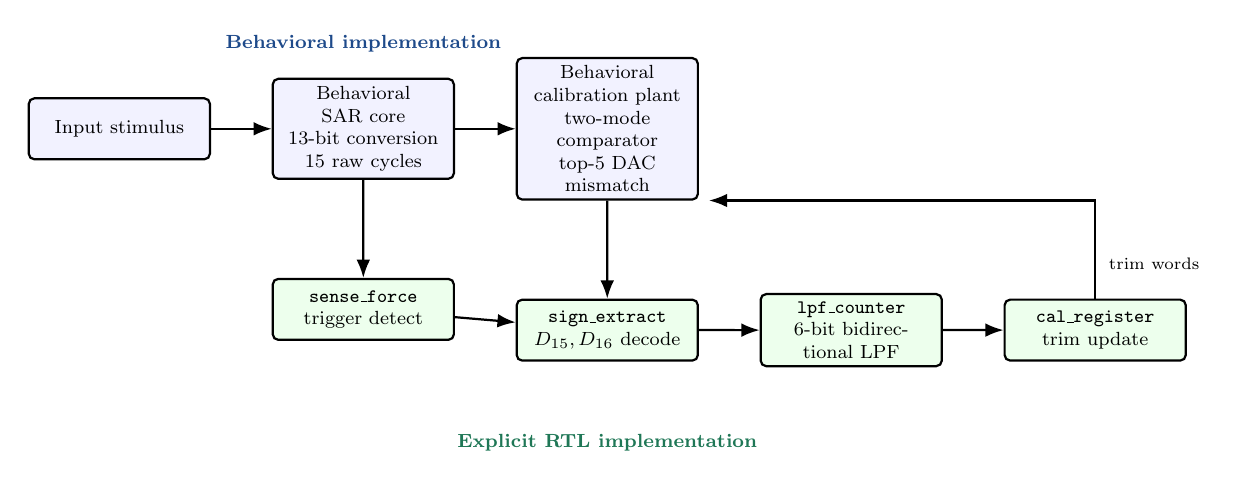
\begin{tikzpicture}[
    scale=0.86,
    transform shape,
    font=\footnotesize,
    >=Latex,
    blk/.style={draw, rounded corners=2pt, thick, minimum height=0.9cm, align=center, text width=2.45cm, inner sep=3.2pt},
    beh/.style={blk, fill=blue!5},
    rtl/.style={blk, fill=green!7},
    arr/.style={->, thick}
]
    \node[beh] (stim) {Input stimulus};
    \node[beh, right=0.9cm of stim] (sar) {Behavioral SAR core\\13-bit conversion\\15 raw cycles};
    \node[beh, right=0.9cm of sar] (plant) {Behavioral calibration plant\\two-mode comparator\\top-5 DAC mismatch};

    \node[rtl, below=1.45cm of sar] (sense) {\texttt{sense\_force}\\trigger detect};
    \node[rtl, below=1.45cm of plant] (sign) {\texttt{sign\_extract}\\$D_{15},D_{16}$ decode};
    \node[rtl, right=0.9cm of sign] (lpf) {\texttt{lpf\_counter}\\6-bit bidirectional LPF};
    \node[rtl, right=0.9cm of lpf] (reg) {\texttt{cal\_register}\\trim update};

    \node[adcblue, font=\bfseries\footnotesize, above=0.25cm of sar] {Behavioral implementation};
    \node[adcgreen, font=\bfseries\footnotesize, below=0.95cm of sign] {Explicit RTL implementation};

    \draw[arr] (stim) -- (sar);
    \draw[arr] (sar) -- (plant);
    \draw[arr] (sar.south) -- (sense.north);
    \draw[arr] (plant.south) -- (sign.north);
    \draw[arr] (sense) -- (sign);
    \draw[arr] (sign) -- (lpf);
    \draw[arr] (lpf) -- (reg);
    \draw[arr] (reg.north) |- ($(plant.south east)+(0.15,0)$);
    \node[font=\scriptsize, anchor=west] at ($(reg.north)+(0.08,0.52)$) {trim words};
\end{tikzpicture}
\caption{Hybrid project architecture. The converter and correction plant remain behavioral, while the sign-extraction and trim-update path are explicitly implemented in RTL.}
\label{fig:top_arch}
\end{figure}

Figure~\ref{fig:sign_flow} shows the implemented sign path in a paper-style cycle-15/cycle-16 view based on the calibration method in \cite{ding2017}. For comparator calibration, the DAC code is held fixed while the comparator mode changes between the two final cycles. For DAC calibration, cycle 16 forces the alternate redundant A/B code. In both cases, the sign logic only examines whether $D_{15}$ and $D_{16}$ differ and converts that difference into the correction direction required by the trim hardware.

\begin{figure}[H]
\centering
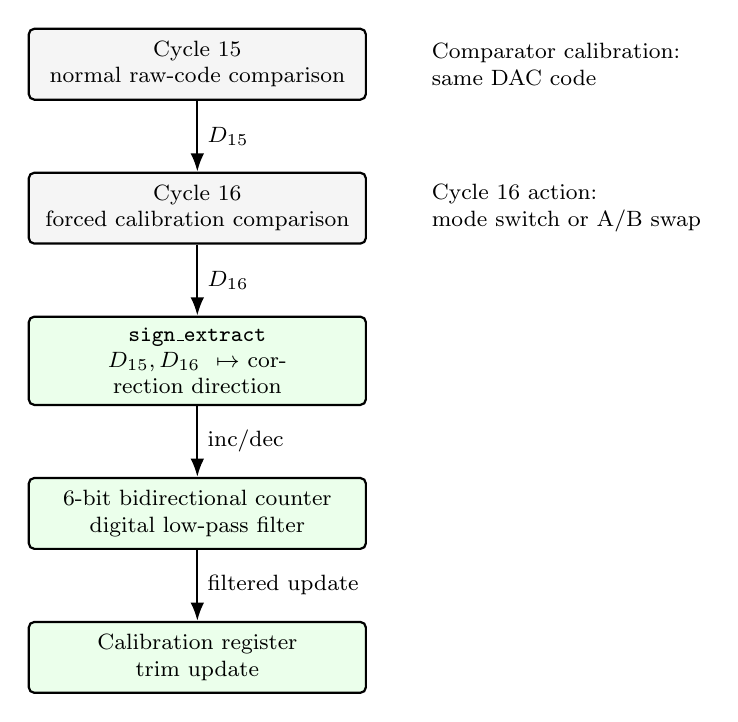
\begin{tikzpicture}[
    font=\footnotesize,
    >=Latex,
    box/.style={draw, rounded corners=2pt, thick, minimum height=0.9cm, align=center, text width=4.0cm, inner sep=4pt},
    arr/.style={->, thick}
]
    \node[box, fill=gray!8] (c15) {Cycle 15\\normal raw-code comparison};
    \node[box, below=0.9cm of c15, fill=gray!8] (c16) {Cycle 16\\forced calibration comparison};
    \node[box, below=0.9cm of c16, fill=green!8] (sgn) {\texttt{sign\_extract}\\$D_{15},D_{16}\mapsto$ correction direction};
    \node[box, below=0.9cm of sgn, fill=green!8] (lpf) {6-bit bidirectional counter\\digital low-pass filter};
    \node[box, below=0.9cm of lpf, fill=green!8] (trim) {Calibration register\\trim update};

    \node[align=left, anchor=west] at ($(c15.east)+(0.7,0.0)$) {Comparator calibration:\\same DAC code};
    \node[align=left, anchor=west] at ($(c16.east)+(0.7,0.0)$) {Cycle 16 action:\\mode switch or A/B swap};

    \draw[arr] (c15) -- node[right]{$D_{15}$} (c16);
    \draw[arr] (c16) -- node[right]{$D_{16}$} (sgn);
    \draw[arr] (sgn) -- node[right]{inc/dec} (lpf);
    \draw[arr] (lpf) -- node[right]{filtered update} (trim);
\end{tikzpicture}
\caption{Implemented sign-extraction path. The logic uses the final two comparison outcomes to determine correction direction, then applies a 6-bit bidirectional counter as the digital LPF described in the paper.}
\label{fig:sign_flow}
\end{figure}

\section{Implemented Blocks}
\subsection{Sense and Force}
The \texttt{sense\_force} block is implemented as a purely combinational decoder. It receives the 15-bit behavioral raw code and splits it into a 7-bit \texttt{x\_code} field and a 3-bit \texttt{y\_code} field. Calibration is permitted only when \texttt{y\_code == 3'b110}, which reproduces the centered background-calibration activation idea described in \cite{ding2017}. Once that gate is met, the block checks the \texttt{x\_code} against one comparator family and five DAC A/B code pairs.

Comparator calibration is selected when \texttt{x\_code[6:2] == 5'b11000}. In that case the block asserts \texttt{cal\_active}, sets \texttt{cal\_mode\_comp = 1}, routes the request to channel 5, and forwards \texttt{x\_code[1]} as \texttt{ab\_sel}. DAC calibration uses ten explicit 7-bit codes, two per channel, covering the top five capacitors. For example, channel 0 uses \texttt{0111111}/\texttt{1000000}, channel 1 uses \texttt{0101111}/\texttt{0110000}, and the remaining channels continue inward toward midscale in the same A/B-pair form. The outputs of this block are therefore not abstract labels; they are the actual control signals used by the rest of the implemented calibration chain.

\subsection{Sign Extraction}
The sign-extraction block is the main non-behavioral requirement of the project, and it is implemented as combinational logic. The block takes five inputs: \texttt{valid}, \texttt{cal\_mode\_comp}, \texttt{ab\_sel}, \texttt{d15}, and \texttt{d16}. In the current implementation the decision rule itself is intentionally compact: if \texttt{valid} is low, or if \texttt{d15} and \texttt{d16} are equal, the block emits no sign information. Only when \texttt{valid \&\& (d15 \string^ d16)} is true does it declare a useful sign event.

Within that valid event window, the block computes
\[
\texttt{sign\_pos} = D_{15}\overline{D_{16}}, \qquad
\texttt{sign\_neg} = \overline{D_{15}}D_{16}.
\]
The outputs \texttt{inc\_i} and \texttt{dec\_i} are then driven directly from \texttt{sign\_pos} and \texttt{sign\_neg}. In other words, the implementation does not calculate an error magnitude and then quantize it. It simply latches the relative ordering of the final two comparison results and converts that ordering into a one-cycle increment or decrement request for the trim loop. The sign convention is therefore tied to the correction direction required by the implemented trim hardware rather than to an abstract algebraic sign.

\begin{table}[H]
\centering
\caption{Implemented sign-extraction mapping.}
\label{tab:signmap}
\begin{tabular}{cccccc}
\toprule
Valid & $D_{15}$ & $D_{16}$ & sign\_valid & inc\_i & dec\_i \\
\midrule
0 & X & X & 0 & 0 & 0 \\
1 & 0 & 0 & 0 & 0 & 0 \\
1 & 1 & 1 & 0 & 0 & 0 \\
1 & 1 & 0 & 1 & 1 & 0 \\
1 & 0 & 1 & 1 & 0 & 1 \\
\bottomrule
\end{tabular}
\end{table}

\subsection{Digital LPF and Trim Update}
The paper's \cite{ding2017} digital low-pass filter is implemented as a 6-bit bidirectional counter, and the project follows that structure directly. Each counter is clocked and resettable, starts at \texttt{INIT = 32}, and ignores contradictory requests. When \texttt{inc\_i} is asserted by itself, the count moves upward by one. When \texttt{dec\_i} is asserted by itself, the count moves downward by one. If the counter reaches one count before either edge, it does not remain saturated; instead it emits a one-cycle filtered update pulse (\texttt{inc\_o} or \texttt{dec\_o}) and immediately reloads to its midpoint. This reproduces the intended effect of requiring many repeated sign decisions before an actual trim change is allowed.

The trim word update is implemented separately as a synchronous saturating register with a 7-bit trim word. On \texttt{inc\_o} it increments by one unless already at all ones, and on \texttt{dec\_o} it decrements by one unless already at zero. In the full project simulation there are six copies of the LPF-plus-register path: five for the DAC capacitor channels and one for the comparator channel. This means the implemented digital portion of the project is not only the sign extractor itself, but the complete chain from trigger detection through filtered trim update.

\section{Behavioral Model}
The converter core and analog correction path remain behavioral. This includes the 13-bit conversion source, the simplified 15-bit redundant raw-code encoding, the two-mode comparator offset plant, the top-five DAC mismatch model, and the analog effect of the trim words. The important improvement over the earliest project model is that $D_{15}$ and $D_{16}$ are now generated from actual behavioral DAC/comparator comparisons rather than from a placeholder signed-error variable, matching the intent of the paper's sign-based loop \cite{ding2017}.

The DAC side uses explicit trim-dependent weight perturbations for the top five capacitors, so a change in trim word directly changes the converter transfer behavior. The comparator side uses two effective operating modes, which allows the calibration loop to act on a mode-dependent offset difference rather than on a single static comparator error. This is still a system-level model, but it is much closer to the implemented calibration mechanism than the earlier placeholder-error version.

\section{Results}
\subsection{Single-Loop Sanity Checks}
Before enabling the full six-channel background loop, simplified single-loop testbenches were used to verify that the explicit sign-extraction path drives the trim in the correct direction. Figure~\ref{fig:simpleloops} shows one comparator-offset case and one DAC case.

These sanity-check plots serve as a digital-path validation step. They confirm that the sign-extraction output, the bidirectional counter, and the trim register all agree on the required correction direction before sparse trigger activation is introduced.

\begin{figure}[H]
\centering
\begin{tikzpicture}
\begin{groupplot}[
    group style={group size=2 by 1, horizontal sep=1.6cm},
    width=0.44\textwidth,
    height=0.28\textwidth,
    grid=both,
    xlabel={Cycle},
    tick label style={font=\footnotesize},
    label style={font=\footnotesize},
    legend style={font=\footnotesize, draw=none, fill=none, at={(0.5,-0.22)}, anchor=north, legend columns=2},
    ymin=0,
    xmin=0
]
\nextgroupplot[title={Comparator-offset loop}, ylabel={Value}]
\addplot[adcblue, thick] table[x=cycle,y=effective_error,col sep=comma] {data/simple_loop_comp.csv};
\addlegendentry{Effective error}
\addplot[adcred, thick, dashed] table[x=cycle,y=trim_word,col sep=comma] {data/simple_loop_comp.csv};
\addlegendentry{Trim word}

\nextgroupplot[title={Representative DAC loop}, ylabel={Value}]
\addplot[adcblue, thick] table[x=cycle,y=effective_error,col sep=comma] {data/simple_loop_dac.csv};
\addlegendentry{Effective error}
\addplot[adcred, thick, dashed] table[x=cycle,y=trim_word,col sep=comma] {data/simple_loop_dac.csv};
\addlegendentry{Trim word}
\end{groupplot}
\end{tikzpicture}
\caption{Single-loop sanity checks used to verify that the implemented sign path moves the trim word in the expected direction.}
\label{fig:simpleloops}
\end{figure}

\subsection{Background Calibration Convergence}
The full background-calibration experiment includes one comparator loop and five DAC loops. Figure~\ref{fig:trimconv} plots the six trim words as the background calibration proceeds. The long settling time is a direct result of sparse trigger-code activation rather than continuous correction on every conversion.

\begin{figure}[H]
\centering
\begin{tikzpicture}
\begin{axis}[
    width=0.88\textwidth,
    height=0.36\textwidth,
    grid=both,
    xlabel={Conversion cycle},
    ylabel={Trim word},
    tick label style={font=\footnotesize},
    label style={font=\footnotesize},
    legend style={font=\footnotesize, at={(0.5,1.03)}, anchor=south, legend columns=3, draw=none, fill=none},
    xmin=0,
    ymin=0,
    ymax=22
]
\addplot[adcblue, thick] table[x=cycle,y=trim0,col sep=comma] {data/background_trim_downsampled.csv};
\addlegendentry{Comparator trim}
\addplot[adcred, thick] table[x=cycle,y=trim1,col sep=comma] {data/background_trim_downsampled.csv};
\addlegendentry{DAC0 trim}
\addplot[adcgreen, thick] table[x=cycle,y=trim2,col sep=comma] {data/background_trim_downsampled.csv};
\addlegendentry{DAC1 trim}
\addplot[adcorange, thick] table[x=cycle,y=trim3,col sep=comma] {data/background_trim_downsampled.csv};
\addlegendentry{DAC2 trim}
\addplot[adcpurple, thick] table[x=cycle,y=trim4,col sep=comma] {data/background_trim_downsampled.csv};
\addlegendentry{DAC3 trim}
\addplot[adcgray, thick] table[x=cycle,y=trim5,col sep=comma] {data/background_trim_downsampled.csv};
\addlegendentry{DAC4 trim}
\end{axis}
\end{tikzpicture}
\caption{Convergence of the six calibration trim words in the full background run.}
\label{fig:trimconv}
\end{figure}

To mimic the paper's Fig.~22 style \cite{ding2017}, Figure~\ref{fig:sndrconv} plots the SNDR obtained by evaluating the implemented DAC-mismatch equations and the implemented two-mode comparator model at the actual trim states recorded during the background-calibration run. The curve therefore comes from the implemented project state trajectory rather than from a fitted proxy. After convergence, the evaluated SNDR settles at approximately \SI{73.8}{dB}.

\begin{figure}[H]
\centering
\begin{tikzpicture}
\begin{axis}[
    width=0.82\textwidth,
    height=0.34\textwidth,
    grid=both,
    xlabel={Time (samples)},
    ylabel={SNDR (dB)},
    tick label style={font=\footnotesize},
    label style={font=\footnotesize},
    xmin=0,
    xmax=400000,
    ymin=60,
    ymax=76,
    xtick={0,100000,200000,300000,400000},
    xticklabels={0,100k,200k,300k,400k}
]
\addplot[adcred, thick, mark=none] table[x=cycle,y=sndr_db,col sep=comma] {data/sndr_vs_cycles.csv};
\node[adcred, anchor=west] at (rel axis cs:0.75,0.90) {Evaluated SNDR};
\end{axis}
\end{tikzpicture}
\caption{SNDR-convergence plot in the style of the paper's Fig.~22, evaluated directly from the implemented dynamic SAR output model using the recorded trim trajectory. The horizontal scale is expressed directly in conversion samples, and the converged SNDR is approximately \SI{73.8}{dB}.}
\label{fig:sndrconv}
\end{figure}

Figure~\ref{fig:spectra} recreates the paper's \cite{ding2017} three-scenario spectrum comparison using the implemented project model: without calibration, with comparator-offset calibration only, and with a fully corrected comparator-plus-DAC trim state. These spectra are evaluated from the same dynamic SAR output model used for Figure~\ref{fig:sndrconv}; however, Figure~\ref{fig:spectra} uses a fair endpoint comparison, while Figure~\ref{fig:sndrconv} shows the actual implemented convergence trajectory.

This distinction is important for interpreting the figures. Figure~\ref{fig:sndrconv} answers how the implemented loop evolves under sparse background updates, whereas Figure~\ref{fig:spectra} compares three specific operating points using a common final-state evaluation method. Taken together, they show both the convergence process and the endpoint spectral behavior.

\begin{figure}[H]
\centering
\begin{tikzpicture}
\begin{groupplot}[
    group style={group size=1 by 3, vertical sep=1.0cm},
    width=0.84\textwidth,
    height=0.20\textwidth,
    grid=both,
    xmin=0,
    xmax=3.2,
    ymin=-120,
    ymax=5,
    ylabel={Magnitude (dBFS)},
    tick label style={font=\footnotesize},
    label style={font=\footnotesize}
]
\nextgroupplot[title={Without calibration}]
\addplot[adcgray, very thick] table[x=freq_mhz,y=dbfs,col sep=comma] {data/spectrum_uncal.csv};
\node[anchor=north east] at (rel axis cs:0.97,0.94) {SNDR = 63.0 dB};

\nextgroupplot[title={With comparator calibration only}]
\addplot[adcorange, very thick] table[x=freq_mhz,y=dbfs,col sep=comma] {data/spectrum_comp_only.csv};
\node[anchor=north east] at (rel axis cs:0.97,0.94) {SNDR = 73.8 dB};

\nextgroupplot[title={With comparator and DAC calibration}, xlabel={Frequency (MHz)}]
\addplot[adcgreen, very thick] table[x=freq_mhz,y=dbfs,col sep=comma] {data/spectrum_both.csv};
\node[anchor=north east] at (rel axis cs:0.97,0.94) {SNDR = 73.9 dB};
\end{groupplot}
\end{tikzpicture}
\caption{Spectrum comparison in the style of the paper's Fig.~19, evaluated from the implemented dynamic SAR output model for three calibration states: without calibration, with comparator calibration only, and with a fully corrected comparator-plus-DAC state.}
\label{fig:spectra}
\end{figure}

The main convergence metrics from the background-calibration run are summarized in Table~\ref{tab:convergence}.

\begin{table}[H]
\centering
\caption{Background calibration convergence summary.}
\label{tab:convergence}
\begin{tabular}{lc}
\toprule
Metric & Result \\
\midrule
Total convergence cycle & 384243 \\
Active calibration events & 5257 \\
Active-event rate & 1.37\% \\
Comparator loop convergence & 299008 \\
DAC0 convergence & 384243 \\
DAC1 convergence & 346060 \\
DAC2 convergence & 252461 \\
DAC3 convergence & 219268 \\
DAC4 convergence & 190316 \\
\bottomrule
\end{tabular}
\end{table}

\section{Discussion}
The most important result is that the calibration no longer converges unrealistically fast. Early project models calibrated on essentially every cycle and derived sign information from a placeholder signed-error variable, so they settled in only tens of cycles. After the trigger logic, bidirectional-counter LPF, and behavioral $D_{15}/D_{16}$ generation were tightened, the convergence moved to the same order as the paper's reported result \cite{ding2017}.

The model is still intentionally behavioral. The trigger set is paper-like rather than a literal reconstruction of the full published table in \cite{ding2017}, and the analog trim effect is linearized. That simplification is deliberate: the project emphasis is on the calibration architecture, especially the explicitly implemented sign-extraction path, not on transistor-level circuit replication.

The present version of the report also keeps the dynamic-performance figures internally consistent. The SNDR-convergence curve and the three comparison spectra are both generated from the same implemented dynamic SAR evaluator, rather than from separate post-fit plotting methods. As a result, the reported SNDR values now match the implemented model rather than an auxiliary proxy.

\section{Conclusion}
This project reimplemented the key calibration architecture of the selected 13-bit SAR ADC paper \cite{ding2017} using a hybrid methodology. The converter, mismatch, comparator modes, and correction path were modeled behaviorally, while the sign extraction and its immediate digital control path were implemented directly in RTL. The final background-calibration loop converges in 384243 conversions with a sparse activation rate of 1.37\%, which places the project in the same regime as the paper's \cite{ding2017} roughly 400k-cycle convergence result.

\begin{thebibliography}{1}
\bibitem{ding2017}
M. Ding, P.-I. Mak, M.-K. Law, S.-W. Sin, and R. P. Martins, ``A 46~\si{\micro\watt} 13-b 6.4-MS/s SAR ADC with background mismatch and offset calibration,'' \emph{IEEE Journal of Solid-State Circuits}, vol. 52, no. 10, pp. 2466--2477, Oct. 2017.
\end{thebibliography}

\end{document}
